\documentclass{article}
\usepackage{hyperref}
\usepackage{graphicx}


\begin{document}

\section{Future work}

We earned great results with our methodology, but the algorithm still can be faster.
In future we would like to optimize further the computational costs and the runtime.
We will continue our research in this direction.
Our goal is to decrease the execution time of our algorithm from $\theta(n^2)$ to $\theta (n*log(n))$. This would mean an even bigger breakthrough in the practical application of the SAT problem. 
\begin{figure}[h]
    \centering
    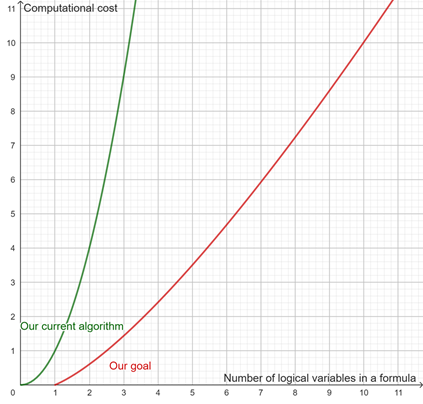
\includegraphics[width=0.5\linewidth]{img/futurework.png}
\end{figure}

\end{document}